\subsection{Data Generation}
\label{sec:soft_cut_data_generation}

The raw data set contains 1,592 soft cut frames and 637,755 non soft cut frames.
% TODO: Wieviele Softcuts sind es genau? Das ist vllt die spannendere Zahl.
This is a very unbalanced ratio which impedes the training.
To achieve a good generalization of a recurrent neural net, we determined that more data was necessary.
% TODO: Hier muss ein Zitat/Referenz stehen, das man bei DL viel Data braucht.
For that, we generated more data by blending random sequences into each other.
The procedure for generating a new random sequence works as follows:
First, we randomly pick two subsequent cuts from the gold standard, each with a start and end frame respectively.
Between the end frame of the first cut and the start frame of the next cut, we can randomly select a subsequence with the desired transition length.
This way, it is guaranteed, that there is no hard cut or soft cut in the random sequence we picked.
Then we do this process again, this time with two other random cuts.
As the result, we now have two randomly selected sequences of the same length, which we can now blend into each other.
In order to blend two random sequences, we have multiple options for tweening behaviour.
The standard tweening function is linear, but we also used ease-in, ease-out and others, see Figure~\ref{fig:data_generation}.
The tweening function is randomly selected, as well.
As the transition type we used a classic \textit{dissolve}.

In order to achieve further variance in the generated data, we flip the two sequences randomly at the x- or y-axis or at both axes.
With this approach we generated about 50 GB of data.
% TODO: Das ist ja jetzt gerade unvergleichbar mit den Zahlen von oben, weil wir oben absolute Zahlen hatten und hier auf einmal GB.
% Das muessen wir noch vereinheitlichen.
% ICh bin dafuer, hier noch die Anzahl der Soft cuts/non soft cuts hinzuschreiben.

\begin{figure}
    \centering
    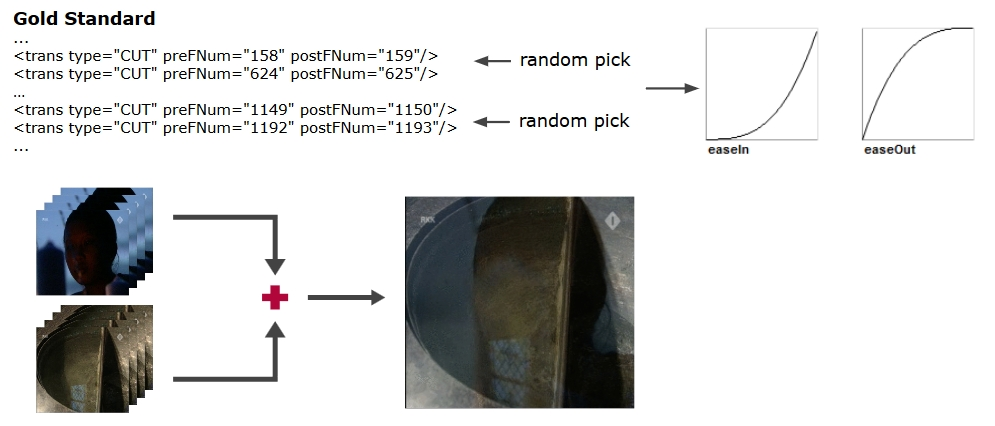
\includegraphics[scale=.5]{images/data_generation.jpg}
    \caption{}
    \label{fig:data_generation}
\end{figure}
% TODO: Figure Text missing.
